\documentclass[journal,12pt,twocolumn]{IEEEtran}

\usepackage{setspace}
\usepackage{gensymb}

\singlespacing


\usepackage[cmex10]{amsmath}

\usepackage{amsthm}

\usepackage{mathrsfs}
\usepackage{txfonts}
\usepackage{stfloats}
\usepackage{bm}
\usepackage{cite}
\usepackage{cases}
\usepackage{subfig}

\usepackage{longtable}
\usepackage{multirow}

\usepackage{enumitem}
\usepackage{mathtools}
\usepackage{steinmetz}
\usepackage{tikz}
\usepackage{circuitikz}
\usepackage{verbatim}
\usepackage{tfrupee}
\usepackage[breaklinks=true]{hyperref}
\usepackage{graphicx}
\usepackage{tkz-euclide}
\usepackage{float}

\usetikzlibrary{calc,math}
\usepackage{listings}
    \usepackage{color}                                            %%
    \usepackage{array}                                            %%
    \usepackage{longtable}                                        %%
    \usepackage{calc}                                             %%
    \usepackage{multirow}                                         %%
    \usepackage{hhline}                                           %%
    \usepackage{ifthen}                                           %%
    \usepackage{lscape}     
\usepackage{multicol}
\usepackage{chngcntr}

\DeclareMathOperator*{\Res}{Res}

\renewcommand\thesection{\arabic{section}}
\renewcommand\thesubsection{\thesection.\arabic{subsection}}
\renewcommand\thesubsubsection{\thesubsection.\arabic{subsubsection}}

\renewcommand\thesectiondis{\arabic{section}}
\renewcommand\thesubsectiondis{\thesectiondis.\arabic{subsection}}
\renewcommand\thesubsubsectiondis{\thesubsectiondis.\arabic{subsubsection}}


\hyphenation{op-tical net-works semi-conduc-tor}
\def\inputGnumericTable{}                                 %%

\lstset{
%language=C,
frame=single, 
breaklines=true,
columns=fullflexible
}
\begin{document}
\newtheorem{theorem}{Theorem}[section]
\newtheorem{problem}{Problem}
\newtheorem{proposition}{Proposition}[section]
\newtheorem{lemma}{Lemma}[section]
\newtheorem{corollary}[theorem]{Corollary}
\newtheorem{example}{Example}[section]
\newtheorem{definition}[problem]{Definition}

\newcommand{\BEQA}{\begin{eqnarray}}
\newcommand{\EEQA}{\end{eqnarray}}
\newcommand{\define}{\stackrel{\triangle}{=}}
\bibliographystyle{IEEEtran}
\providecommand{\mbf}{\mathbf}
\providecommand{\pr}[1]{\ensuremath{\Pr\left(#1\right)}}
\providecommand{\qfunc}[1]{\ensuremath{Q\left(#1\right)}}
\providecommand{\sbrak}[1]{\ensuremath{{}\left[#1\right]}}
\providecommand{\lsbrak}[1]{\ensuremath{{}\left[#1\right.}}
\providecommand{\rsbrak}[1]{\ensuremath{{}\left.#1\right]}}
\providecommand{\brak}[1]{\ensuremath{\left(#1\right)}}
\providecommand{\lbrak}[1]{\ensuremath{\left(#1\right.}}
\providecommand{\rbrak}[1]{\ensuremath{\left.#1\right)}}
\providecommand{\cbrak}[1]{\ensuremath{\left\{#1\right\}}}
\providecommand{\lcbrak}[1]{\ensuremath{\left\{#1\right.}}
\providecommand{\rcbrak}[1]{\ensuremath{\left.#1\right\}}}
\theoremstyle{remark}
\newtheorem{rem}{Remark}
\newcommand{\sgn}{\mathop{\mathrm{sgn}}}
\providecommand{\abs}[1]{\vert#1\vert}
\providecommand{\res}[1]{\Res\displaylimits_{#1}} 
\providecommand{\norm}[1]{\lVert#1\rVert}
%\providecommand{\norm}[1]{\lVert#1\rVert}
\providecommand{\mtx}[1]{\mathbf{#1}}
\providecommand{\mean}[1]{E[ #1 ]}
\providecommand{\fourier}{\overset{\mathcal{F}}{ \rightleftharpoons}}
%\providecommand{\hilbert}{\overset{\mathcal{H}}{ \rightleftharpoons}}
\providecommand{\system}{\overset{\mathcal{H}}{ \longleftrightarrow}}
	%\newcommand{\solution}[2]{\textbf{Solution:}{#1}}
\newcommand{\solution}{\noindent \textbf{Solution: }}
\newcommand{\cosec}{\,\text{cosec}\,}
\providecommand{\dec}[2]{\ensuremath{\overset{#1}{\underset{#2}{\gtrless}}}}
\newcommand{\myvec}[1]{\ensuremath{\begin{pmatrix}#1\end{pmatrix}}}
\newcommand{\mydet}[1]{\ensuremath{\begin{vmatrix}#1\end{vmatrix}}}
\numberwithin{equation}{subsection}
\makeatletter
\@addtoreset{figure}{problem}
\makeatother
\let\StandardTheFigure\thefigure
\let\vec\mathbf
\renewcommand{\thefigure}{\theproblem}
\def\putbox#1#2#3{\makebox[0in][l]{\makebox[#1][l]{}\raisebox{\baselineskip}[0in][0in]{\raisebox{#2}[0in][0in]{#3}}}}
     \def\rightbox#1{\makebox[0in][r]{#1}}
     \def\centbox#1{\makebox[0in]{#1}}
     \def\topbox#1{\raisebox{-\baselineskip}[0in][0in]{#1}}
     \def\midbox#1{\raisebox{-0.5\baselineskip}[0in][0in]{#1}}
\vspace{3cm}
\title{ASSIGNMENT 1}
\author{Dishank Jain \\ AI20BTECH11011}
\maketitle
\newpage
\bigskip
\renewcommand{\thefigure}{\theenumi}
\renewcommand{\thetable}{\theenumi}
Download all latex-tikz codes from 
%
\begin{lstlisting}
https://github.com/Dishank422/EE3900/blob/main/Gate-Assignment1/latex_code.tex
\end{lstlisting}
%
\section{EC 2019 Q.33}
Let the state-space representation on an LTI system be $\dot{x}(t) = Ax(t)+Bu(t)$, $y(t)=Cx(t)+du(t)$ where A,B,C are matrices,  d is a scalar, u(t) is the input to the system, and y(t) is its output. Let $B = \begin{pmatrix} 0 & 0 &  1\end{pmatrix}^\top$ and $d = 0$. Which one of the following options for A and C will ensure that the transfer function of this LTI system is 
\begin{equation}
    H(s) = \dfrac{1}{s^3+3s^2+2s+1}
\end{equation}

\begin{enumerate}[label = (\Alph*)]
    \item $A = \begin{pmatrix}
     0 &  1 &  0\\ 
     0 &  0 &  1\\
    -1 & -2 & -3
    \end{pmatrix}$ and $C = \begin{pmatrix}1 & 0 & 0\end{pmatrix}$
    \item $A = \begin{pmatrix}
     0 &  1 &  0\\ 
     0 &  0 &  1\\
    -3 & -2 & -1
    \end{pmatrix}$ and $C = \begin{pmatrix}1 & 0 & 0\end{pmatrix}$
    \item $A = \begin{pmatrix}
     0 &  1 &  0\\ 
     0 &  0 &  1\\
    -1 & -2 & -3
    \end{pmatrix}$ and $C = \begin{pmatrix}0 & 0 & 1\end{pmatrix}$
    \item $A = \begin{pmatrix}
     0 &  1 &  0\\ 
     0 &  0 &  1\\
    -3 & -2 & -1
    \end{pmatrix}$ and $C = \begin{pmatrix}0 & 0 & 1\end{pmatrix}$
\end{enumerate}

\section{Solution}

By definition, the transfer function is given by 
\begin{equation}
    H(s) = \dfrac{Y(s)}{U(s)}
\end{equation}
where Y(s) and U(s) are the Laplace transforms of y(t) and u(t) respectively, i.e.
\begin{equation}
    Y(s) = \mathcal{L}(y(t)); \;U(s) = \mathcal{L}(u(t))
\end{equation}

\begin{equation}
    Let \; Y(s) = Z(s)
    \label{z}
\end{equation}
\begin{equation}
    \implies U(s) = (s^3+3s^2+2s+1)Z(s)
\end{equation}
\begin{equation}
    Let \;\mathcal{L}^{-1}(Z(s)) = z(t)
\end{equation}
\begin{multline}
    \implies \mathcal{L}^{-1}(U(s)) = \mathcal{L}^{-1}(s^3Z(s))+\mathcal{L}^{-1}(3s^2Z(s))+\\\mathcal{L}^{-1}(2sZ(s))+\mathcal{L}^{-1}(Z(s))
\end{multline}
\begin{equation}
     \implies u(t) = \dddot{z}(t)+3\ddot{z}(t)+2\dot{z}(t)+z(t)
     \label{3ddiffeq}
\end{equation}

Equation \ref{3ddiffeq} is a linear third degree ordinary differential equation. We can convert this into a system of first order differential equations as follows.
\begin{align}
    Let\; x_1 &= z\\
    x_2 &= \dot{x}_1 = \dot{z}\\
    x_3 &= \dot{x}_2 = \ddot{z}\\
    \implies \dot{x}_3 &= \dddot{z} = u - 3x_3 - 2x_2 - x_1
\end{align}

\begin{align}
    \implies \dot{x}(t) &= \begin{pmatrix} \dot{x}_1\\\dot{x}_2\\\dot{x_3}\end{pmatrix} \\
                        &= \begin{pmatrix} x_2\\x_3\\u-3x_3-2x_2-x1\end{pmatrix}\\
                        &= \begin{pmatrix}0 & 1 & 0\\ 0 & 0 & 1 \\ -1 & -2 & -3 \end{pmatrix} \begin{pmatrix}x_1\\x_2\\x_3\end{pmatrix}+\begin{pmatrix}0 \\ 0 \\ 1\end{pmatrix}u\\
                        &= \begin{pmatrix}0 & 1 & 0\\ 0 & 0 & 1 \\ -1 & -2 & -3 \end{pmatrix}x(t) + \begin{pmatrix}0 \\ 0 \\ 1\end{pmatrix}u(t)
\end{align}

We know that $\dot{x}(t) = Ax(t)+Bu(t)$ and $B = \begin{pmatrix} 0 & 0 &  1\end{pmatrix}^\top$. Hence on comparison
\begin{equation}
    A = \begin{pmatrix}0 & 1 & 0\\ 0 & 0 & 1 \\ -1 & -2 & -3 \end{pmatrix}
\end{equation}

Also, since $d=0$, 
\begin{equation}
    y(t)= Cx(t)+du(t) = Cx(t)
\end{equation}
But from \ref{z}, 
\begin{align}
    \mathcal{L}^{-1}(Y(s)) &= \mathcal{L}^{-1}(Z(s))\\
    \implies y(t) &= z(t)\\
                  &= x_1\\
                  &= \begin{pmatrix}1 & 0 & 0\end{pmatrix} \begin{pmatrix}x_1\\x_2\\x_3\end{pmatrix}\\
                  &= \begin{pmatrix}1 & 0 & 0\end{pmatrix}x(t)\\
    \implies C &= \begin{pmatrix}1 & 0 & 0\end{pmatrix}
\end{align}

Hence option (A) is the correct option.
%\begin{figure}[!h]
%         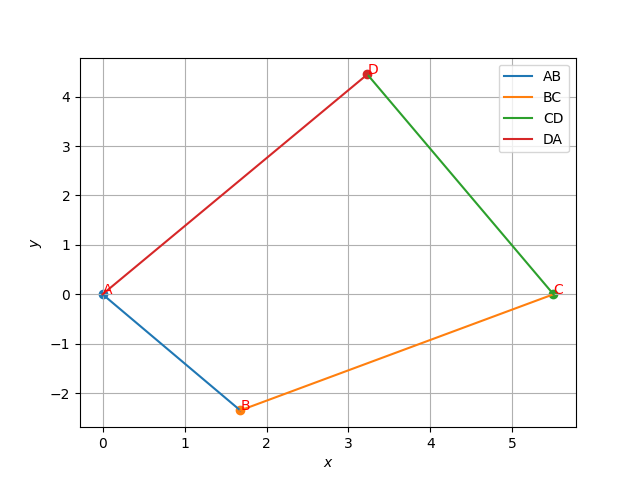
\includegraphics[width=\columnwidth]{figure.png}
%         \caption{Plot of the line}
%         \label{plot}
%\end{figure}
\end{document}
